\documentclass[12pt, a5paper, french]{memoir}
\usepackage[bottom=91pt]{geometry}
\usepackage[utf8]{inputenc}
\usepackage[T1]{fontenc}
\usepackage{lmodern}
\usepackage{microtype}
\usepackage{dramatist}
\usepackage[modulo]{lineno}
\usepackage{hyperref}
\usepackage{graphicx}
\usepackage{babel}

\renewcommand{\actname}{Acte}
\renewcommand{\scenename}{Scène}
\renewcommand{\printscenenum}{\scenenumfont \thescene}
\renewcommand{\casttitlename}{Personnages}

\makepagestyle{myps}
\makeevenfoot{myps}{\thepage}{}{}
\makeoddfoot{myps}{}{}{\thepage}

\title{L'anneau de Gygès}
\author{Alexandre \textsc{Pachot}\thanks{Texte sous licence \href{http://creativecommons.org/licenses/by-sa/4.0/deed.fr}{CC BY-SA}, inspiré d’une fable racontée dans la \textit{République} de Platon.}}

\hyphenation{Michel-angelo}

\begin{document}
\maketitle
\vfill
\begin{figure}[h]
\centering
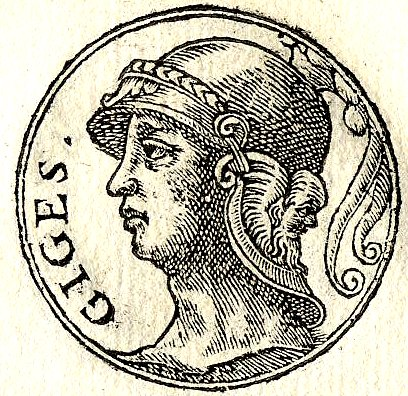
\includegraphics[scale=1]{Gyges.jpg}
\end{figure}
\vfill
\thispagestyle{empty}
\newpage
\renewcommand\contentsname{Sommaire}
\tableofcontents*

\Character[Gygès]{Gygès}{Gyges}
\Character[Candaule, le roi]{Candaule}{Candaule}
\Character[Nyssia, la fiancée du roi]{Nyssia}{Nyssia}
\Character[Laurel, un serviteur du roi]{Laurel}{Laurel}
\Character[Hardy, un serviteur de Nyssia]{Hardy}{Hardy}
\Character[Bonnie, une voleuse]{Bonnie}{Bonnie}
\Character[Clyde, un voleur]{Clyde}{Clyde}
\Character[Leonardo, un berger]{Leonardo}{Leonardo}
\Character[Donatello, un berger]{Donatello}{Donatello}
\Character[Michelangelo, un berger]{Michelangelo}{Michelangelo}
\Character[Raffaello, un berger]{Raffaello}{Raffaello}
\Character[Tiziano, un berger]{Tiziano}{Tiziano}
   
\DramPer*
\pagestyle{myps}
\linenumbers
\scene

\StageDir{\Gyges, \Bonnie, \Clyde}
\begin{drama}
\Bonniespeaks Connais-tu la dernière nouvelle ?
\Clydespeaks Quelle nouvelle ?
\Bonniespeaks Le roi vient de s’acheter la dernière Nintendo, la 3DS~XXL.
\Clydespeaks Comment sais-tu ça ?
\Bonniespeaks C’est écrit dans le journal. Si seulement tu savais lire\dots
\Clydespeaks Pff ! Le journal, il suffit de le regarder à la télé !
\Bonniespeaks Au lieu de dire des bêtises, dis-moi plutôt comment on va faire pour voler cette console.
\Clydespeaks \direct{Apercevant quelqu’un au loin.} C’est qui là-bas ?
\Bonniespeaks C’est Gygès, au pied de son arbre, en train de surveiller ses chèvres.
\Clydespeaks Allons le saluer. \direct{À Gygès.} Gygès, tu viens avec nous, on va élaborer un plan pour dérober la dernière console du roi.
\Gygesspeaks Moi, Monsieur, je suis honnête, je respecte les lois, je ne vole pas.
\Bonniespeaks Gygès, au lieu de faire le malin, réponds plutôt à la question suivante : tu ne voles pas, car tu as peur de te faire arrêter, ou parce que tu es l’incarnation même de la justice ? Si tu avais de super-pouvoirs tout en étant certain de ne pas te faire attraper, que ferais-tu ? Respecterais-tu la loi, ou pas ? Là, tu fais moins le malin ! Bon, je te laisse, moi j’ai du travail à faire, il faut qu’on trouve un plan pour s’emparer de cette console !

\scene

\StageDir{\Gyges}
\Gygesspeaks \direct{Scrutant le pied de l’arbre.} Un affaissement ? Je ne l’avais jamais remarqué. On dirait qu’il y a quelque chose au fond. Tiens, une boite ? Il y a un texte écrit dessus : \og Ô mortel, garde-toi d’envier le bonheur d’aucun autre homme. \fg{} \direct{Ouvre la boite.} Tout cela pour un anneau ! \direct{Passe la bague à son doigt, le chaton à l’extérieur.} Bon, rien ne se passe ! Ce n’est pas tout, mais il faut que je retourne au village, il y a le conseil des bergers.

\scene

\StageDir{\Gyges, \Leonardo, \Donatello, \Michelangelo, \Raffaello, \Tiziano}
\Leonardospeaks \direct{Apercevant Gygès} Gygès, dépêche-toi, cela fait des lustres qu’on t’attend. On n’a pas que ça à faire. J’ai des pommes de terre à éplucher.
\Donatellospeaks Oh ! On est ici pour parler de chèvres, pas de patates !
\Michelangelospeaks Bon. Qui va voir le roi pour faire un rapport sur l'état des troupeaux ?
\Raffaellospeaks Pas moi.
\Tizianospeaks Moi.
\Donatellospeaks Non, pas toi. La dernière fois, tu as eu un problème avec le roi.
\Leonardospeaks Bon, alors c’est Gygès qui va aller voir le roi.
\Gygesspeaks \direct{À lui-même.} Je vais tourner le chaton de ma bague vers l’intérieur, voir ce que cela fait.
\Leonardospeaks Il est où Gygès ? Saperlipopette, il a encore disparu.
\Raffaellospeaks C’est vrai, ça. Il était encore là, il y a 5~secondes.
\Gygesspeaks \direct{Tournant le chaton vers l’extérieur.} Les amis, c’est moi que vous cherchez ?
\Tizianospeaks Ah ! Te voilà enfin de retour. Bon, nous avons décidé que c’est toi qui vas aller voir le roi pour lui faire un rapport sur nos troupeaux.
\Gygesspeaks D’accord, je m’en vais de ce pas, voir le roi.

\scene

\StageDir{\Gyges, \Candaule, \Nyssia, \Laurel}
\Laurelspeaks Votre Majesté, Gygès vient d’arriver.
\Candaulespeaks Bien, faites-le entrer.
\Gygesspeaks Votre Majesté.
\Candaulespeaks Gygès, mon ami, comment vont les affaires ?
\Gygesspeaks Bien.
\Candaulespeaks Avant de parler affaires, il faut que je te présente ma nouvelle fiancée. Passe un peu de temps avec elle et dis-moi ce que tu en penses.
\Gygesspeaks Votre Majesté, cela serait indécent\dots
\Candaulespeaks J’insiste. \direct{À Nyssia.} Nyssia, viens voir ici. Je dois partir, j’ai des affaires à régler. Je te présente Gygès, un ami qui va te tenir compagnie pour le diner.

\scene

\StageDir{\Gyges, \Nyssia, \Hardy}
\Gygesspeaks \direct{À lui-même.} J’ai bien mangé. Il en a de la chance le roi, d’épouser une si belle fille. Je l’envie.
\Hardyspeaks \direct{À Nyssia.} Mon altesse, je viens d’apprendre que le roi est furieux de la conduite de Gygès. Il veut le tuer.
\Nyssiaspeaks Vite, va prévenir Gygès du sort qui l’attend.
\Hardyspeaks \direct{À Gygès.} Monsieur, vous courez un grand danger, le roi veut votre mort.
\Gygesspeaks Ha ! Le scélérat ! Je vais utiliser mon anneau d’invisibilité pour le tuer pendant son sommeil.

\scene

\StageDir{\Bonnie, \Clyde}
\Bonniespeaks Connais-tu la dernière nouvelle ?
\Clydespeaks Quelqu’un a volé la console du roi ?
\Bonniespeaks Non ! Le roi a été assassiné. Maintenant, c’est Gygès qui est roi à la place du roi.
\Clydespeaks Le roi est mort, vive le roi !
\Bonniespeaks Mais cela ne répond pas à la question.
\Clydespeaks Quelle question ?
\Bonniespeaks Si l’on était protégé de la conséquence de nos actes, est-ce qu’on agirait de la même manière ?
\end{drama}

\hfill
\centering

\textsc{Fin}
\end{document}